\subsection{Example}

\begin{frame}{Task}
\begin{columns}
    
\begin{column}{0.5\textwidth}

\scriptsize
    Implement a data validation algorithm using SHA512.
    
    Algorithm procedure:
    \begin{enumerate}
        \item Tile the input file into blocks of 1MB. (If the last block is smaller than 1MB, pad it with zeros.)
        \item For the $i^{th}$ block, concatenate it with the validation sum SHA512 of $(i-1)^{th}$ block and calculate validation sum of SHA512.
        \item The validation sum of the last block is considered as the validation sum of the entire file.
    \end{enumerate}

    \textbf{Source}: HPC Game 2024
\end{column}

\begin{column}{0.5\textwidth}
    \begin{figure}
        \centering
        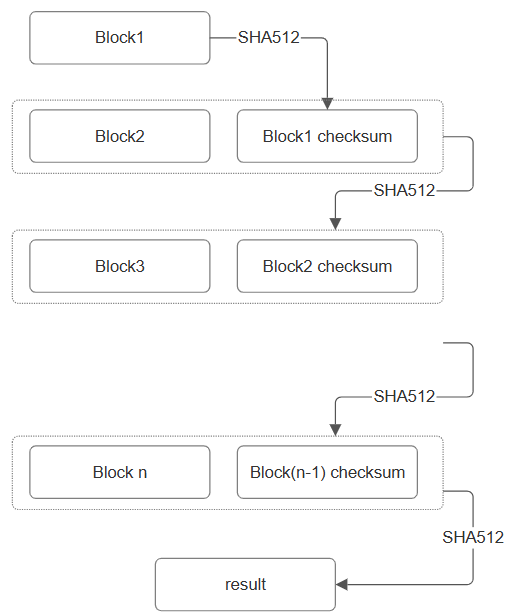
\includegraphics[width=0.65\linewidth]{day8_am/img/mpi/SHA512.png}
    \end{figure}
\end{column}
\end{columns}
\end{frame}

\begin{frame}[fragile]{Baseline Code}
    \begin{columns}
    \begin{column}{.5\textwidth}
\begin{minted}[fontsize=\tiny]{c}
int num_block = (len + BLOCK_SIZE - 1) / BLOCK_SIZE;
uint8_t prev_md[SHA512_DIGEST_LENGTH];

EVP_MD_CTX *ctx = EVP_MD_CTX_new();
EVP_MD *sha512 = EVP_MD_fetch(nullptr, "SHA512", nullptr);

SHA512(nullptr, 0, prev_md);
\end{minted}
        \end{column}
        
        \begin{column}{.5\textwidth}
        \begin{minted}[fontsize=\tiny]{c}
for (int i = 0; i < num_block; i++) {
    uint8_t buffer[BLOCK_SIZE]{};
    EVP_DigestInit_ex(ctx, sha512, nullptr);
    std::memcpy(buffer, data + i * BLOCK_SIZE,
                std::min(BLOCK_SIZE, len - i * BLOCK_SIZE));
    EVP_DigestUpdate(ctx, buffer, BLOCK_SIZE);
    EVP_DigestUpdate(ctx, prev_md, SHA512_DIGEST_LENGTH);

    unsigned int len = 0;
    EVP_DigestFinal_ex(ctx, prev_md, &len);
}
              \end{minted}
        
        \begin{block}{\scriptsize Notice}
        \scriptsize
            EVP\_DigestUpdate(a);
            EVP\_DigestUpdate(b);
            
            Equivalent to EVP\_DigestUpdate(concate(a,b)) !
        \end{block}
        \end{column}

    \end{columns}
    
\end{frame}

\begin{frame}{Analysis}
    Computation is dependent on the result of the previous one.
    
    How to exploit MPI?

\end{frame}

\begin{frame}{Analysis}
    Computation is dependent on the result of the previous one.
    
    How to exploit MPI?

    \vspace{1cm}

    \textbf{Answer:}
    
    File \textbf{I/O} accounts! We can \textbf{overlap} I/O operations with computation.
\end{frame}

\begin{frame}[fragile]{MPI Code}
    \begin{columns}
    \begin{column}{.5\textwidth}
        \textbf{\scriptsize Non-Blocking receives the previous block's checksum.}
            \begin{minted}[fontsize=\tiny]{c}
if(i != 0) {
  MPI_Irecv((void *)prev_md,
          SHA512_DIGEST_LENGTH,
          MPI_UINT8_T,
          sender,
          0,
          MPI_COMM_WORLD,
          &request);
}
              \end{minted}
        \end{column}
        
        \begin{column}{.5\textwidth}
        \textbf{\scriptsize Meanwhile... File I/O and Digest}
                \begin{minted}[fontsize=\tiny]{c}
istrm.seekg(i * BLOCK_SIZE);
istrm.read(reinterpret_cast<char *>(data + i * BLOCK_SIZE), std::min(BLOCK_SIZE*local_size, file_size - i * BLOCK_SIZE));

for(int j=i; j<upper_bound; j++){
    uint8_t buffer2[BLOCK_SIZE]{};
    EVP_DigestInit_ex(ctx[j-i], sha512, nullptr);
    std::memcpy(buffer2, data + j * BLOCK_SIZE,
                std::min(BLOCK_SIZE, len - j * BLOCK_SIZE));
    EVP_DigestUpdate(ctx[j-i], buffer2, BLOCK_SIZE);
}

if(i != 0){
    MPI_Wait(&request, MPI_STATUS_IGNORE);
}
              \end{minted}
        \end{column}
        
    \end{columns}
    
\end{frame}

\begin{frame}[fragile]{MPI Code (cont.)}
    \begin{columns}
    \begin{column}{.45\textwidth}
        \textbf{\scriptsize Non-blocking send my checksum}
        \begin{minted}[fontsize=\tiny]{c}
unsigned int len = 0;
for(int j=i; j<upper_bound; j++){
    EVP_DigestUpdate(ctx[j-i], prev_md, SHA512_DIGEST_LENGTH);
    EVP_DigestFinal_ex(ctx[j-i], prev_md, &len);
}
if(upper_bound != num_block) {
    MPI_Isend(prev_md,
        SHA512_DIGEST_LENGTH,
        MPI_UINT8_T,
        recepient,
        0,
        MPI_COMM_WORLD,
        &request);
}
              \end{minted}
        \end{column}
        
        \begin{column}{.55\textwidth}
        \begin{figure}
            \centering
            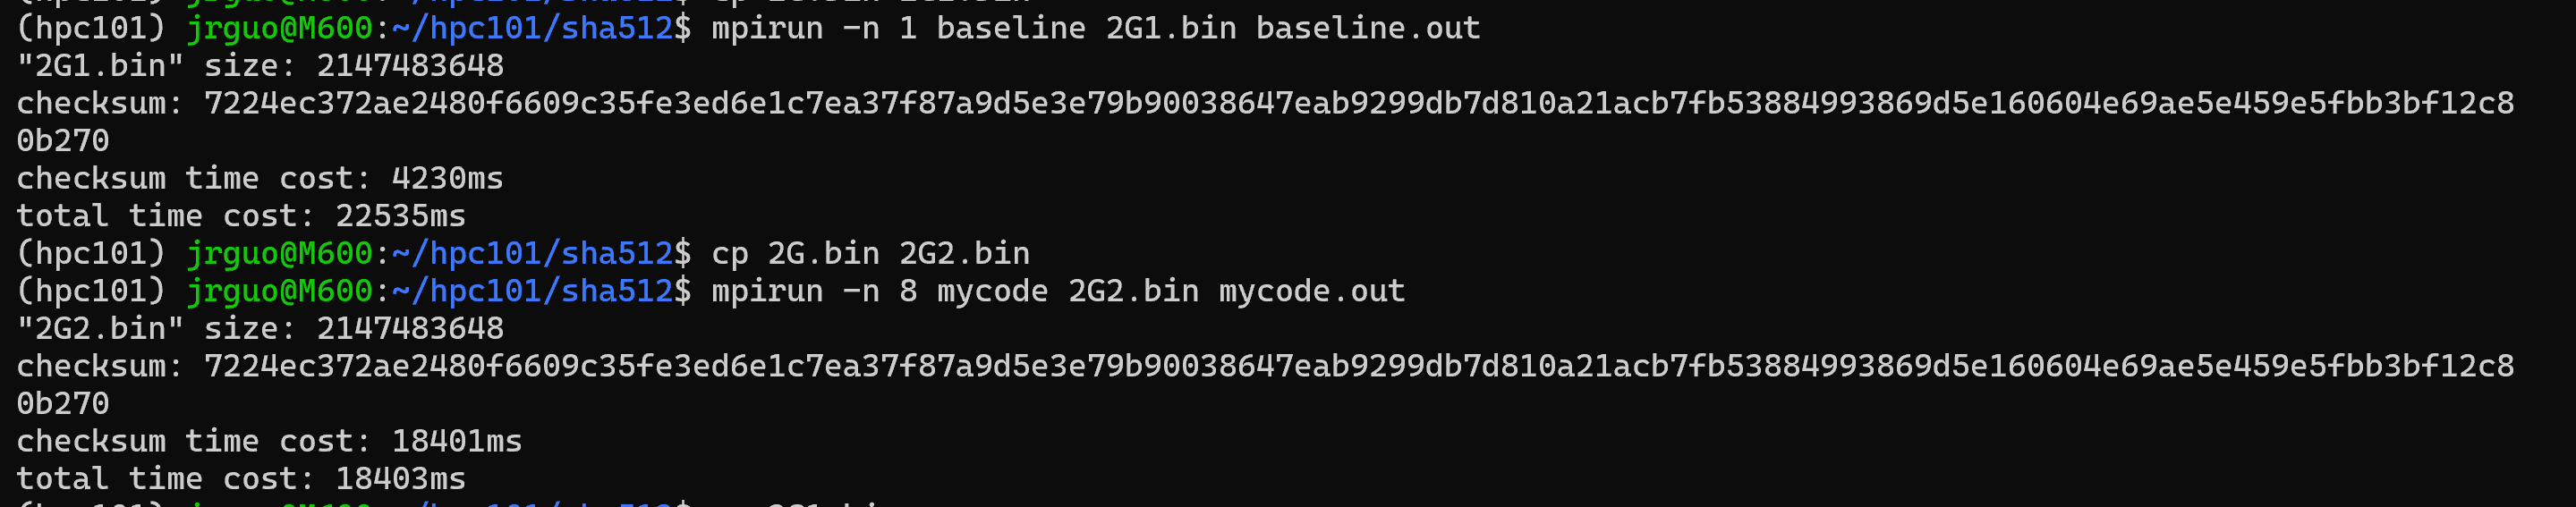
\includegraphics[width=1.0\linewidth]{day8_am/img/mpi/speedup.png}
        \end{figure}

        \vspace{0.5cm}

        \end{column}
        
    \end{columns}
    
\end{frame}

\begin{frame}{Wrap up}
    \begin{figure}
            \centering
            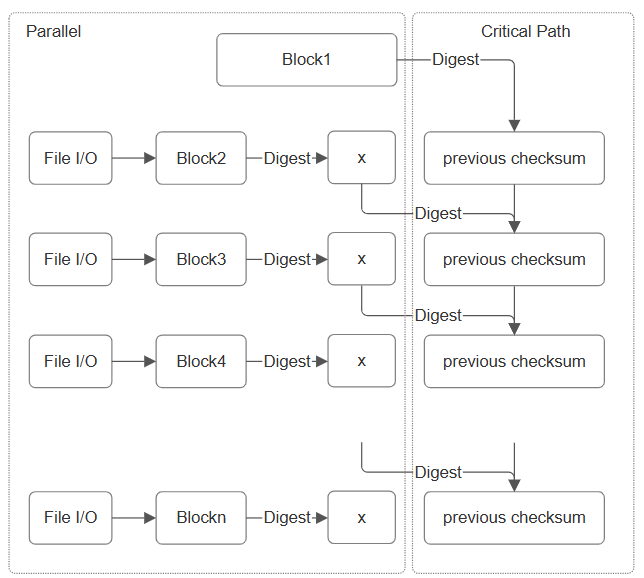
\includegraphics[width=0.45\linewidth]{day8_am/img/mpi/SHA512para.png}
    \end{figure}
\end{frame}
